% !TeX encoding = UTF-8
% !TeX program = pdfLaTeX
% !TeX root = matlab-exercises-emaip.tex
% !TeX spellcheck = en_GB
\section{From old exam sets}



% 2020-02-24 Reexam
\begin{ex}
Reproduce the following figure.
\begin{center}
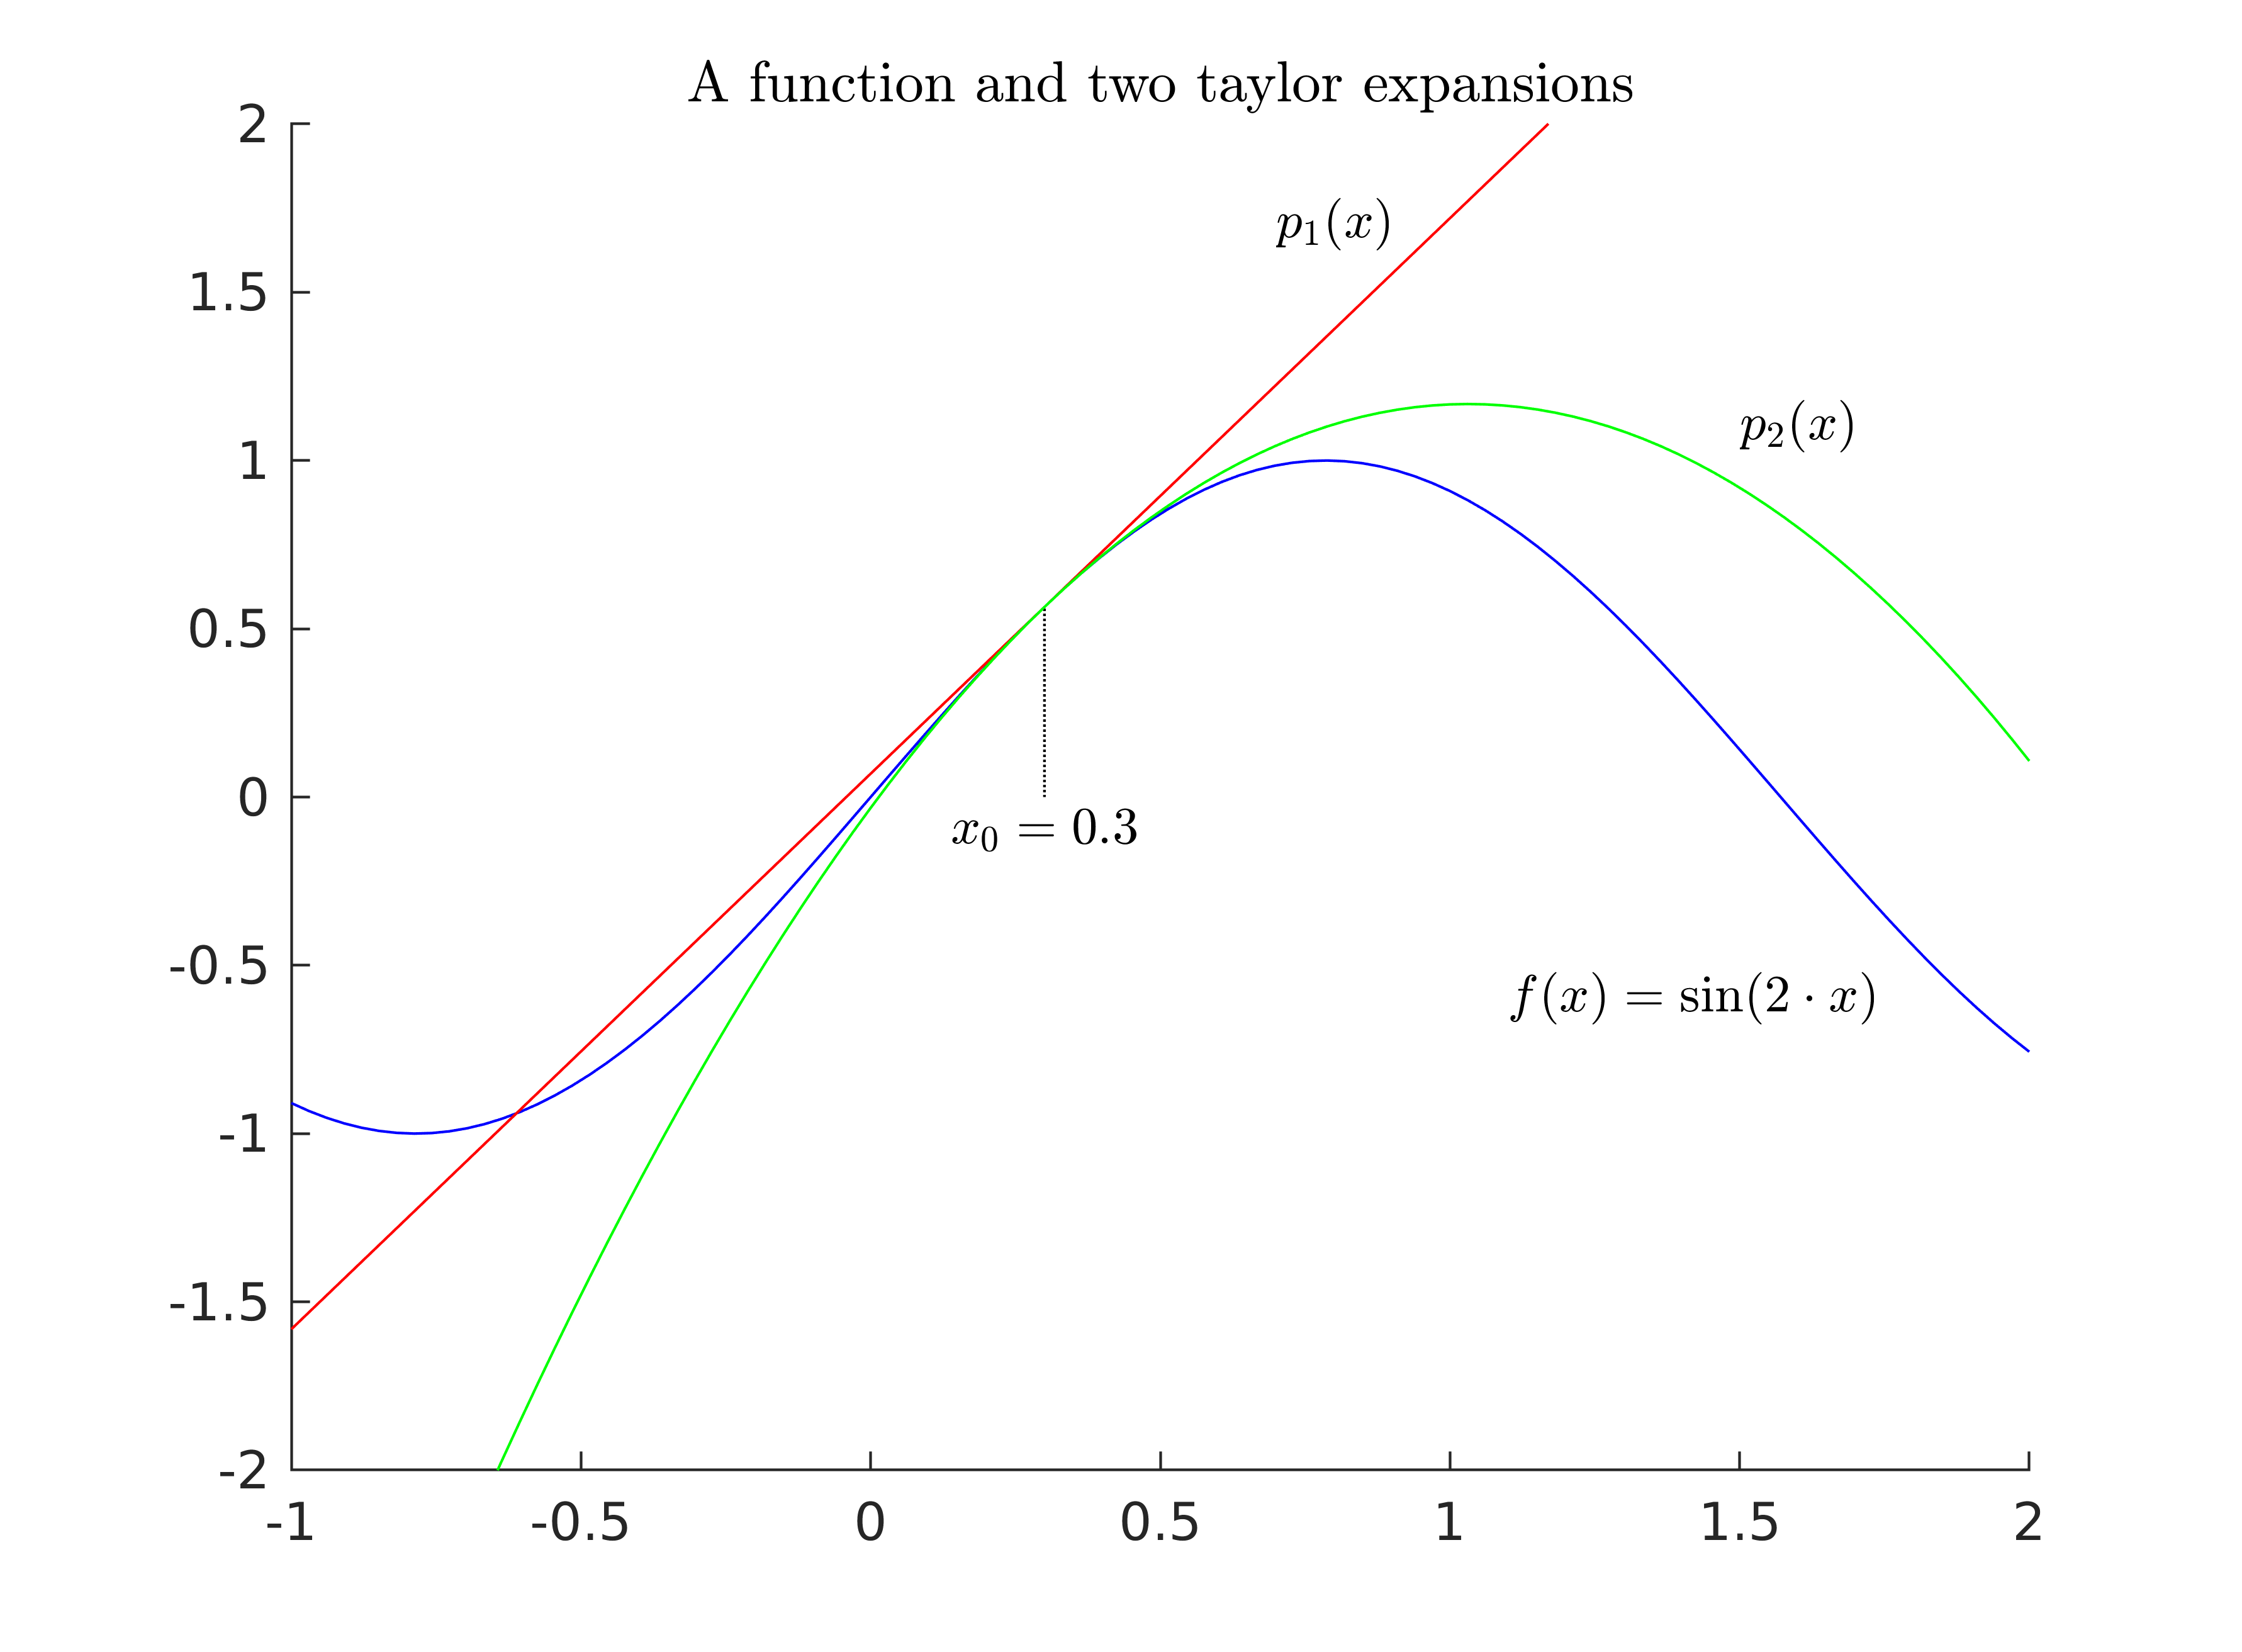
\includegraphics[width=0.7\textwidth]{pic/a_function_and_two_taylorexansions.png}
\end{center}
\begin{hint}
\end{hint}
\begin{sol}
A solution is:
\begin{lstlisting}
%%
xvals = linspace(-1, 2);

fh = @(x) sin(2*x);
dfh = @(x) 2*cos(2*x);
ddfh = @(x) -4*sin(2*x);
x0 = 0.3;

figure(1);
clf;
hold on;
plot(xvals, fh(xvals), 'b')
plot(x0*[1, 1], fh(x0) * [0, 1], 'k:');
plot(xvals, fh(x0)+dfh(x0)*(xvals - x0), 'r')
plot(xvals, fh(x0)+dfh(x0)*(xvals - x0) + 1/2*ddfh(x0)*(xvals - x0).^2, 'g')
ylim([-2, 2])

text(1.1, -0.6, "$f(x) = \sin(2 \cdot x)$", "Interpreter", "latex");
text(0.7, 1.7, "$p_1(x)$", "Interpreter", "latex");
text(1.5, 1.1, "$p_2(x)$", "Interpreter", "latex");
text(0.3, -0.1, "$x_0 = 0.3$", "Interpreter", "latex", ...
     "HorizontalAlignment", "center");
 
title("A function and two taylor expansions", ...
     "Interpreter", "latex");
 
print('a_function_and_two_taylorexansions.png', '-dpng', '-r600');
\end{lstlisting}
\end{sol}
\end{ex}


\begin{ex}
Solve the following five equations with five unknowns:
\begin{align*}
a + b + c + d + e & = 10 \\
a - b + c - d + e & = 6 \\
a + b - c - d - e & = 3 \\
a - b + c & = 3 \\
d + e & = 0
\end{align*}
\begin{hint}
Write the system of equations on extended matrix form
and apply Gaussian elimination.
Then read off the solution.
\end{hint}
\begin{sol}
A solution is:
\begin{lstlisting}
% Enter the linear equations in expanded matrix form.
A = [1, 1, 1, 1, 1, 10; ...
     1, -1, 1, -1, 1, 6; ...
     1, 1, -1, -1, -1, 3; ...
     1, -1, 1, 0, 0, 3; ...
     0, 0, 0, 1, 1, 0];
solution = rref(A)
det(A(:, 1:5))
\end{lstlisting}
\end{sol}
\end{ex}


\begin{ex}
Create a function that calculates the sum of the 
integers from 1 to $n$ raised to a given power $p$.
The function signature should be:
\begin{lstlisting}
function res = sum_of_powers(n, p)
\end{lstlisting}
The input parameters are the last number to include in the 
sum ($n$) and the power to which the integers should be raised ($p$).

The value of \verb!sum_of_powers(4, 3)! is 100
and can be determined through the calculations:
\begin{align*}
\sum_{k = 1}^4 k^3 = 1^3 + 2^3 + 3^3 + 4^3 = 1 + 8 + 27 + 64 = 100
\end{align*}

Use the following examples to test the function:
\begin{lstlisting}
>> sum_of_powers(1, 1)
ans = 1
>> sum_of_powers(4, 1)
ans = 10
>> sum_of_powers(2, 2)
ans = 5
>> sum_of_powers(4, 2)
ans = 30
>> sum_of_powers(10, 1)
ans = 55
>> sum_of_powers(10, 2)
ans = 385
>> sum_of_powers(10, 3)
ans = 3025
\end{lstlisting}
\begin{hint}
\end{hint}
\begin{sol}
A solution is:
\begin{lstlisting}
\end{lstlisting}
\begin{solutionfile}{sum_of_powers_test.m}
%%
function tests = sum_of_powers_test
    tests = functiontests(localfunctions);
end
 

%% Test 1: Positive integer powers of two
function test1(testCase)
    actual_value = sum_of_powers(1, 1);
    expected_value = 1;
    testCase.verifyEqual(actual_value, expected_value);
end

function test2(testCase)
    actual_value = sum_of_powers(1, 2);
    expected_value = 1;
    testCase.verifyEqual(actual_value, expected_value);
end

function test3(testCase)
    actual_value = sum_of_powers(2, 1);
    expected_value = 3;
    testCase.verifyEqual(actual_value, expected_value);
end

function test4(testCase)
    actual_value = sum_of_powers(2, 2);
    expected_value = 5;
    testCase.verifyEqual(actual_value, expected_value);
end

function test5(testCase)
    actual_value = sum_of_powers(10, 1);
    expected_value = 55;
    testCase.verifyEqual(actual_value, expected_value);
end

function test6(testCase)
    actual_value = sum_of_powers(10, 2);
    expected_value = 385;
    testCase.verifyEqual(actual_value, expected_value);
end

function test7(testCase)
    actual_value = sum_of_powers(10, 3);
    expected_value = 3025;
    testCase.verifyEqual(actual_value, expected_value);
end
\end{solutionfile}
\begin{solutionfile}{sum_of_powers.m}
function res = sum_of_powers(n, p)

res = 0;
for k = 1:n
   val = k^p;
   res = res + val;
end

end
\end{solutionfile}
\end{sol}
\end{ex}





% 2020-05-xx
\begin{ex}
Recreate the figure below
\begin{center}
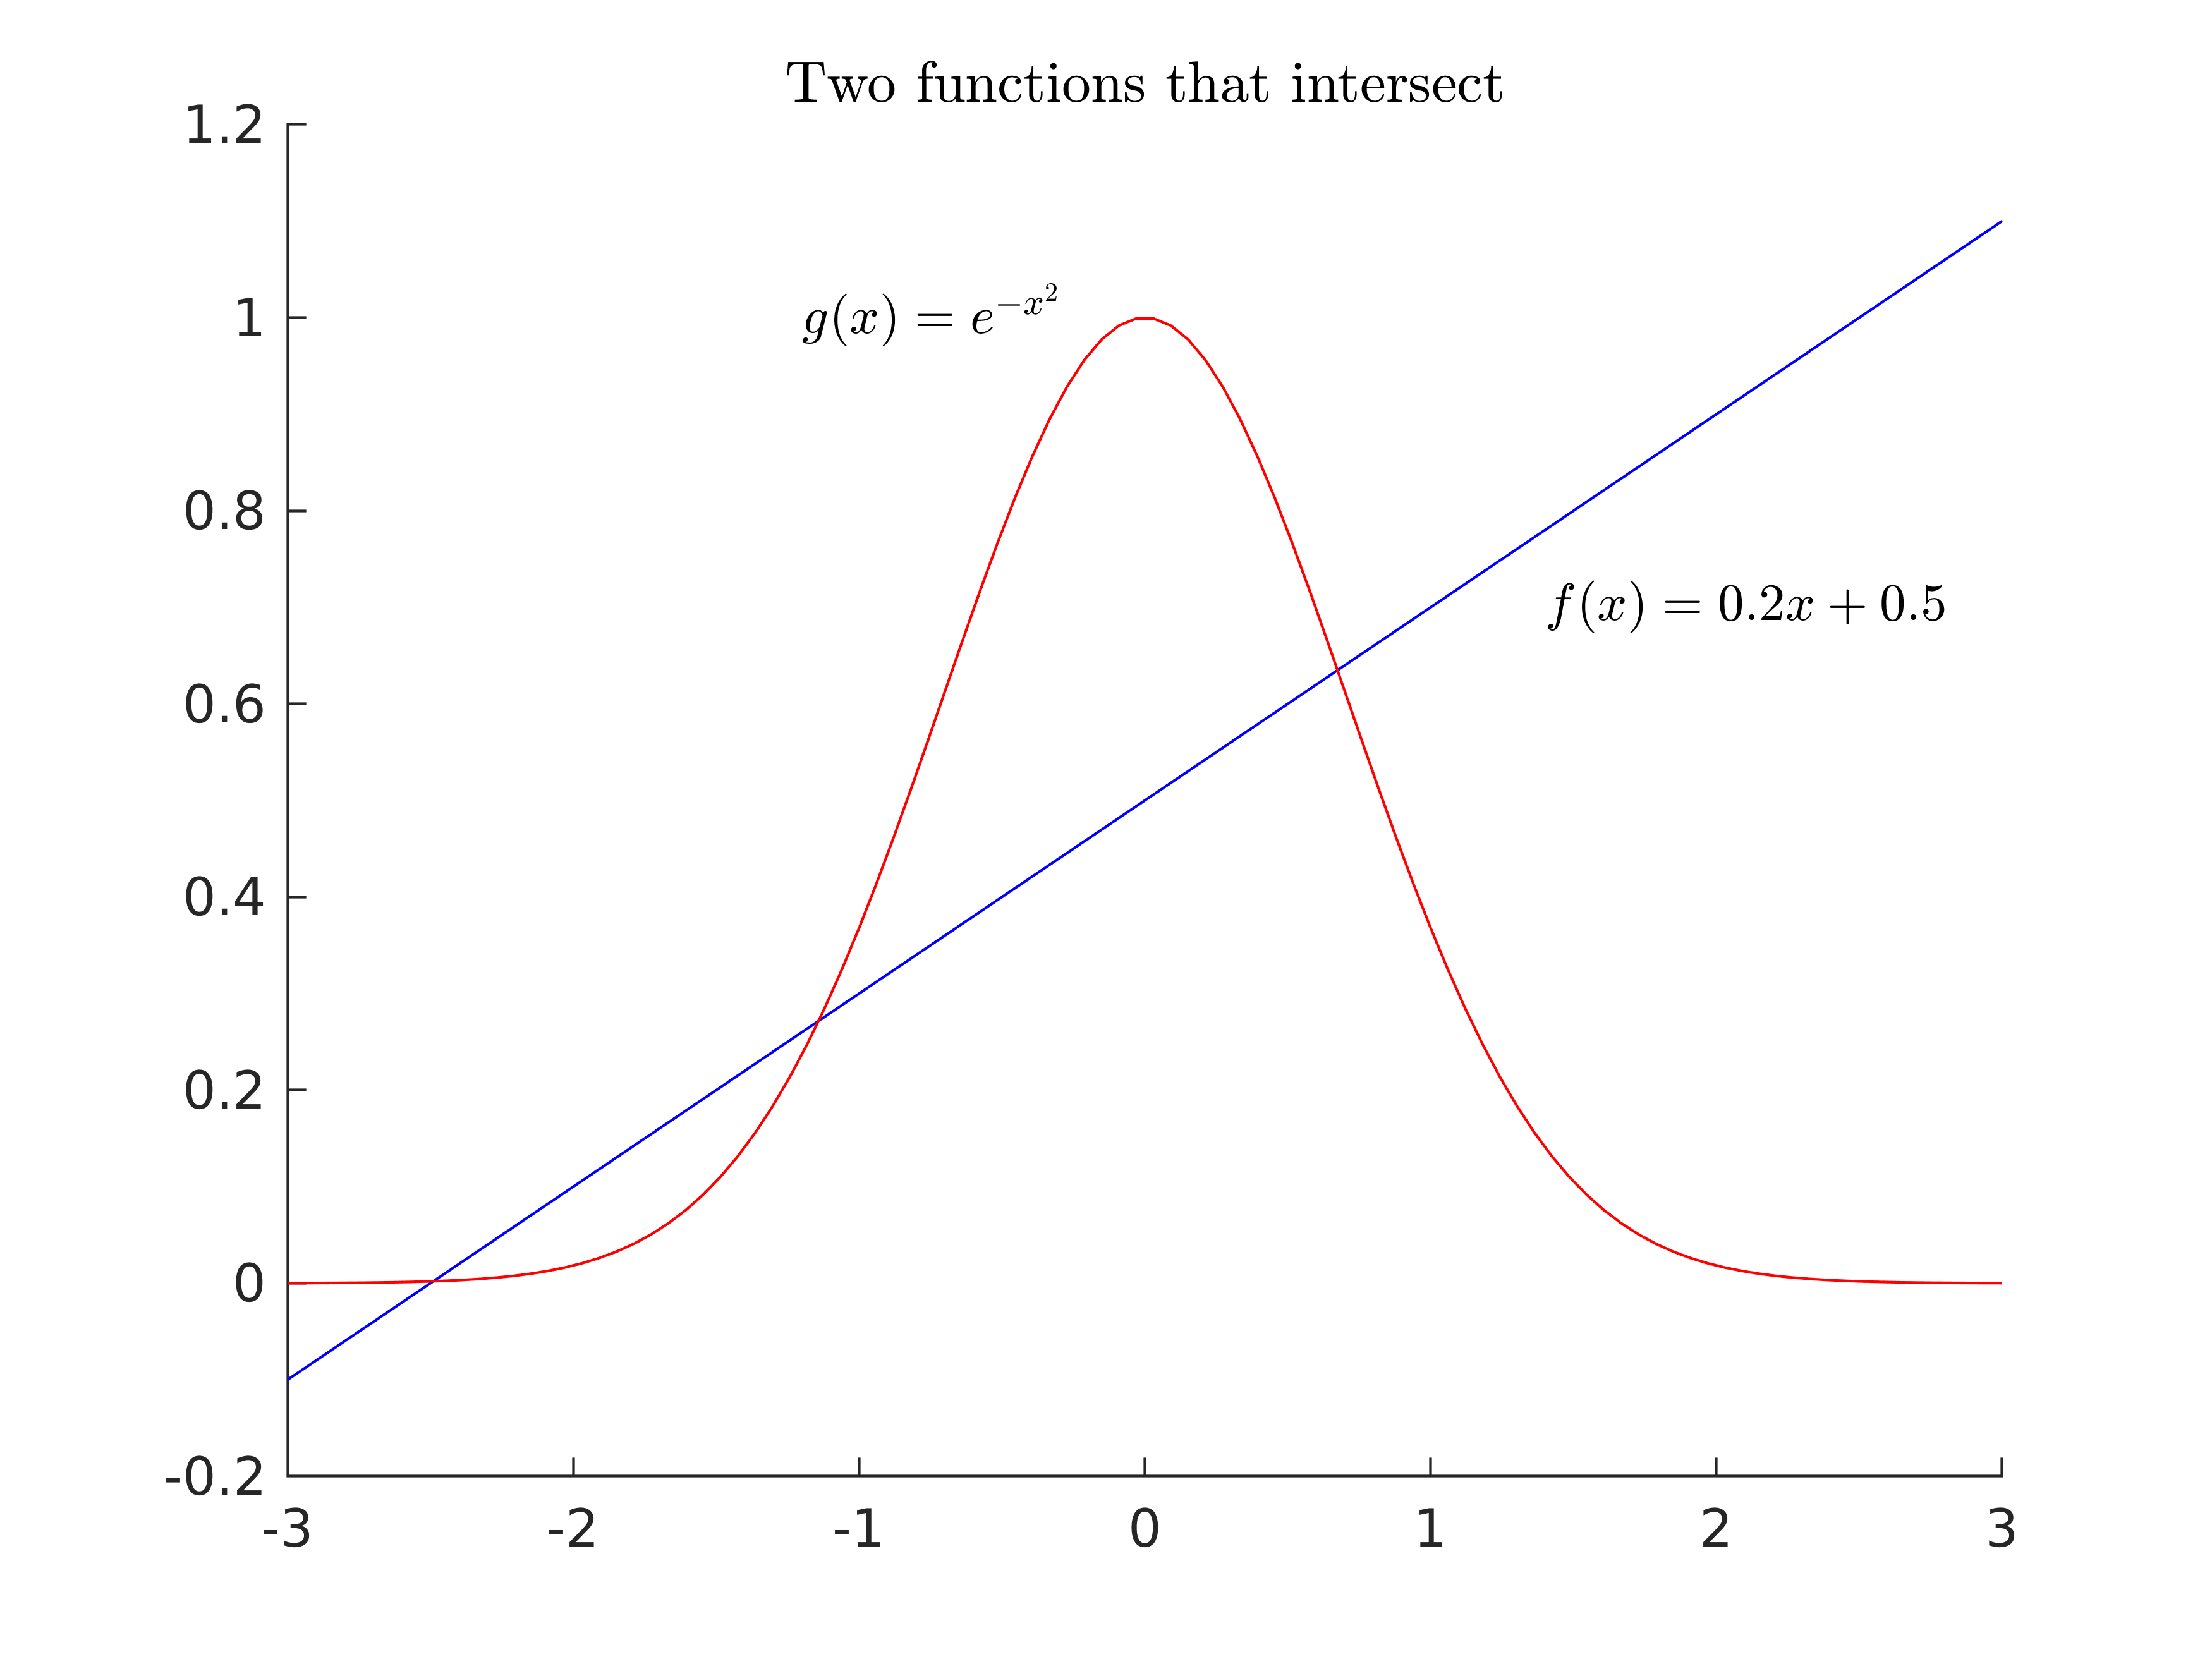
\includegraphics[width=0.7\textwidth]{pic/intersection_of_two_functions.png}
\end{center}
\begin{hint}
\end{hint}
\begin{sol}
A solution is:
\begin{lstlisting}
%%
xvals = linspace(-3, 3);

fh = @(x) 0.2*x + 0.5;
gh = @(x) exp(-x.^2);

figure(1);
clf;
hold on;
plot(xvals, fh(xvals), 'b')
plot(xvals, gh(xvals), 'r')
ylim([-0.2, 1.2])

text(1.4, 0.7, "$f(x) = 0.2 x + 0.5$", "Interpreter", "latex");
text(-1.2, 1.0, "$g(x) = e^{-x^2}$", "Interpreter", "latex");
 
title("Two functions that intersect", ...
     "Interpreter", "latex");
 
print('intersection_of_two_functions.png', '-dpng', '-r600');
\end{lstlisting}
\end{sol}
\end{ex}



\begin{ex}
The following equation has three real solutions:
\begin{align*}
e^{-x^2} = 0.2x + 0.5
\end{align*}
Find these three solutions.
\begin{hint}
\end{hint}
\begin{sol}
A solution is:
\begin{lstlisting}
%%
% Define functions
fh = @(x) 0.2*x + 0.5;
gh = @(x) exp(-x.^2);
hh = @(x) fh(x) - gh(x);

% Search for zeros
r1 = fzero(hh, -2.4)
r2 = fzero(hh, -1)
r3 = fzero(hh, 2)
\end{lstlisting}
\end{sol}
\end{ex}


\begin{ex}
Determine the value of the integral:
\begin{align*}
\int_{-2}^{3} e^{-x^2} dx
\end{align*}
\begin{hint}
\end{hint}
\begin{sol}
A solution is:
\begin{lstlisting}
% Calculate integral
integral(@(x) exp(-x.^2), -2, 3)
\end{lstlisting}
\end{sol}
\end{ex}


\begin{ex}
Implement a function that calculates the area of a triangle 
given the lengths of the three sides using Heron's rule.
Heron's rule is as follows:
Denote the side lengths $a$, $b$ and $c$ and calculate 
the half perimeter:
\begin{align*}
s = \frac{a + b + c}{2}
\end{align*}
Now the area can be calculated through the expression:
\begin{align*}
\textrm{areal} = \sqrt{(s - a) \cdot (s - b) \cdot (s - c) \cdot s}
\end{align*}
The function signature should be:
\begin{lstlisting}
function area = heron(a, b, c)
\end{lstlisting}
The input to the function is the three side lengths
and the value to return is the calculated area.
Eg. is the value of \verb!heron(3, 4, 5)! determined through
the following calculations:
\begin{align*}
s & = \frac{a + b + c}{2} \\ 
& = \frac{3 + 4 + 5}{2} \\
& = 6 \\
\textrm{areal} & = \sqrt{(s - a) \cdot (s - b) \cdot (s - c) \cdot s} \\
& = \sqrt{(6 - 3) \cdot (6 - 4) \cdot (6 - 5) \cdot 6} \\
& = \sqrt{36} = 6
\end{align*}
Use the following examples to test the function:
\begin{lstlisting}
>> heron(3, 4, 5)
ans = 6
>> heron(6, 8, 10)
ans = 24
>> heron(3, 3, 3)
ans = 3.8971
>> heron(3, 3, 6)
ans = 0
>> heron(4, 5, 6)
ans = 9.9216
>> heron(4, 4, 0)
ans = 0
\end{lstlisting}
\begin{hint}
\end{hint}
\begin{sol}
A solution is:
\begin{lstlisting}
\end{lstlisting}
\end{sol}
\end{ex}
 